\begin{solution}
 \begin{enumerate}

\item The given finite difference scheme in $x$ and $t$ can be written as
\[
\frac{u^{j+1}_i - u^j_i}{dt} = \frac{u_{i+1}^j - 2u_i^j + u_{i-1}^j}{h^2}.
\]
 or alternatively,
 \[
u^{j+1}_i = (1-2r) u_{i}^j + r(u_{i+1}^j + u_{i-1}^j).
\]
for $i=1,2 \cdot N$ where $r=\frac{dt}{h^2}$. The matrix system resulting from these equations for homogeneous boundary conditions is
\[
 \underbrace{\left[\begin{array}{c} u_1^{j+1} \\[0.25em] u_2^{j+1} \\[0.25em] \vdots \\[0.25em] u_{N_1}^{j+1} \\[0.25em] u_N^{j+1} \end{array}\right]}_{U^{j+1}}
 =\underbrace{\left[\begin{array}{rrrrr}
              1-2r & r \\[0.25em]
               r & 1-2r & r \\
                 &  r  & 1-2r & \ddots \\
                 & & \ddots & \ddots & 1 \\[0.25em]
                 & & & r & 1-2r 
               \end{array}\right]}_{A}
          \underbrace{\left[\begin{array}{c} u_1^{j} \\[0.25em] u_2^{j}  \\[0.25em] \vdots \\[0.25em] u_{N-1}^{j}  \\[0.25em] u_N^k\end{array}\right]}_{U^j},
\]
Note that for $U^0$ we know the solution by initial conditions. To find the solution next time step we simply need to solve $A U^0 = U^{1}$. We will find $U^1$. In Matlab solving this linear system successively we are able to find solution at $j+1$ time step,i.e.;  $A U^j = U^{j+1}$, we can get solutions for the next time steps.

Included is Matlab code that can be used to generate the finite difference solution for successive time steps:
\lstinputlisting{heatequation_p4.m}
\begin{figure}
\centering
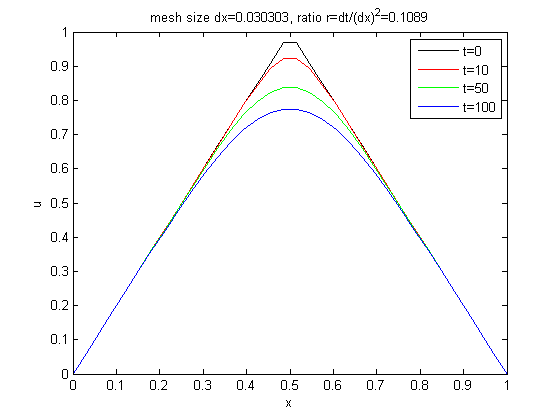
\includegraphics[width=.8\textwidth]{p4a_sol.png}
\caption{Finite difference solutions at various timesteps.}
\end{figure}
\begin{figure}
\centering
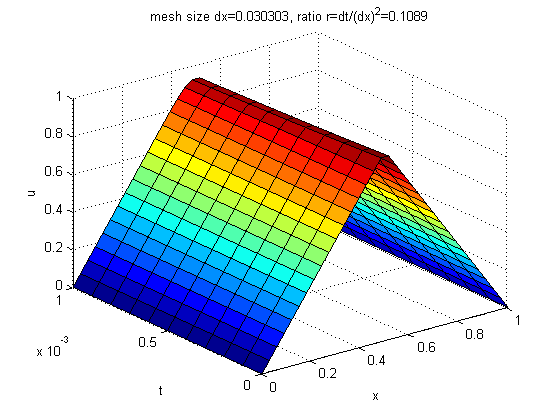
\includegraphics[width=.8\textwidth]{p4a_surf10.png}
\caption{Surface plot for finite difference solution at timestep $10$.}
\end{figure}

\begin{figure}
\centering
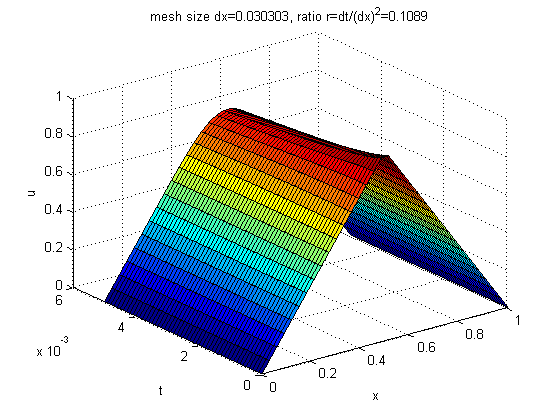
\includegraphics[width=.8\textwidth]{p4a_surf50.png}
\caption{Surface plot for finite difference solution at timestep $50$.}
\end{figure}

\begin{figure}
\centering
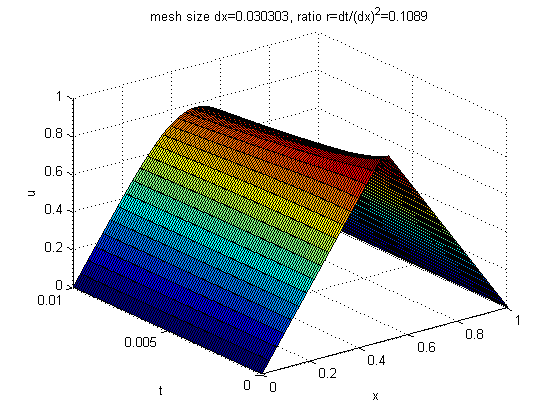
\includegraphics[width=.8\textwidth]{p4a_surf100.png}
\caption{Surface plot for finite difference solution  at timestep $100$.}
\end{figure}

Notice that when we advance in time we get more smooth solutions in other word sharp corner of initial condition turn out parabolic shape. Also there is another fact that we might notice solution is decreasing when $t \rightarrow \infty$. One of the interesting properties of the heat equation is the maximum principle that says ``if $u$ satisfies the heat equation for $0 < x <1$ and $0 < t < T$ then the maximum value of $u$ occurs at $t = 0$ (at the initial
condition) or for $x = 0$ or $x = 1$ (at the boundary point)''. 

\emph{Note: Students does not have to add both 2D plot or 3D surface. One of the plot should be enough.}
 \end{enumerate}
\end{solution}